
\section{Precle}
\index{węzeł!preclowy|see {precel}}%
\index{precel|(}%
Precle to sploty ze standardowym diagramem, na którym wyróżnić można co najmniej trzy warkocze na dokładnie dwóch pasmach.
Warkocze te ułożone są w sposób cykliczny.
Pojawiły się po raz pierwszy w~książce Reidemeistera z~1932 roku jako przykład węzła o~trywialnym wielomianie Alexandera.
Zanim podamy formalną definicję, wygodnie będzie przyjrzyć się ogólniejszej rodzinie splotów Montesinosa, nazwanych tak na cześć José Marii Montesinosa Amilibii, topologa hiszpańskiego.
\index[persons]{Montesinos, José}%
Wprowadził je do matematyki w~1973 roku \cite{montesinos73}.

Kawauchi \cite[s. 29]{kawauchi96} pisze, że Montesinos uogólnił precle, bo dwukrotne nakrycie nad $S^3$ rozgałęzione wzdłuż precla jest rozmaitością Seiferta.
\index{rozmaitość Seiferta}%

\index{splot!Montesinosa|(}%
\begin{definition}[splot Montesinosa]
    Splotem Montesinosa nazywamy splot o~poniższym diagramie, gdzie wymierne liczby $\alpha_i/\beta_i$ oraz całkowita $e \in \Z$ odpowiadają supłom.
\begin{comment}
    \[
    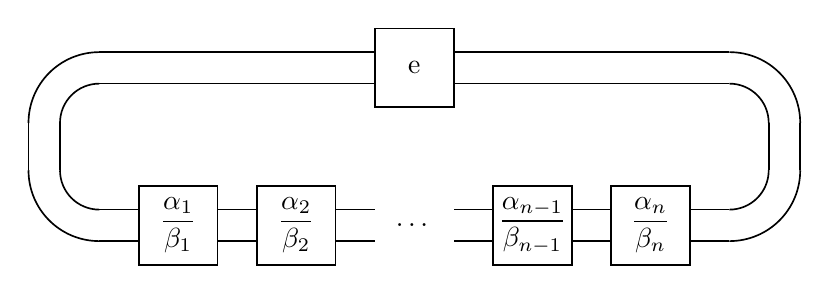
\begin{tikzpicture}[baseline=-0.65ex, scale=0.1]
    %\useasboundingbox (-5, -9) rectangle (5, 5);
        \draw[semithick] (-5, 5) rectangle (5, 15);
        \foreach \x in {0,1,3,4} {
            \draw[semithick] (15*\x-35, -15) rectangle (15*\x-25, -5);
        }
        \foreach \x in {0,1,2,3,4,5} {
            \draw[semithick] (15*\x-35, -8) to (15*\x-40, -8);
            \draw[semithick] (15*\x-35, -12) to (15*\x-40, -12);
        }
        \draw[semithick] (-40, -8) [in=down, out=left] to (-45, -3);
        \draw[semithick] (-40, -12) [in=down, out=left] to (-49, -3);

        \draw[semithick] (-40, 8) [in=up, out=left] to (-45, 3);
        \draw[semithick] (-40, 12) [in=up, out=left] to (-49, 3);

        \draw[semithick] (40, 8) [in=up, out=right] to (45, 3);
        \draw[semithick] (40, 12) [in=up, out=right] to (49, 3);

        \draw[semithick] (40, -8) [in=down, out=right] to (45, -3);
        \draw[semithick] (40, -12) [in=down, out=right] to (49, -3);

        \draw[semithick] (-45, -3)  to (-45, 3);
        \draw[semithick] (-49, -3)  to (-49, 3);
        \draw[semithick] (45, -3)  to (45, 3);
        \draw[semithick] (49, -3)  to (49, 3);

        \draw[semithick] (-5, 8)  to (-40, 8);
        \draw[semithick] ( 5, 8)  to ( 40, 8);
        \draw[semithick] (-5, 12)  to (-40, 12);
        \draw[semithick] ( 5, 12)  to ( 40, 12);

        \node at (0, 10) {e};
        \node at (0, -10) {\ldots};
        \node at (-15, -10) {$\displaystyle \frac{\alpha_2}{\beta_2}$};
        \node at (-30, -10) {$\displaystyle \frac{\alpha_1}{\beta_1}$};
        \node at (15, -10) {$\displaystyle \frac{\alpha_{n-1}}{\beta_{n-1}}$};
        \node at (30, -10) {$\displaystyle \frac{\alpha_n}{\beta_n}$};
    \end{tikzpicture}
    \]
\end{comment}
\end{definition}

Cały dwunasty rozdział podręcznika Burdego i~Zieschanga \cite{burde14} jest poświęcony splotom Montesinosa.
Można tam znaleźć ich klasyfikację, zawiera jednak pułapkę: autorzy używają innej notacji dla supłów dwumostowych.
Podają przykład węzła $43/105 = [0, 2, 2, 3, 1, 4]$, dla nas to jest $105/22 = [4, 1, 3, 2, 2]$.

\begin{proposition}
    Sploty Montesinosa o $r \ge 3$ supłach $\beta_1/\alpha_1, \beta_2/\alpha_2, \ldots$ takich, że
    \begin{equation}
        \sum_{j=1}^r \frac{1}{\alpha_j} \le r - 2
    \end{equation}
    są sklasyfikowane (z dokładnością do cyklicznych permutacji oraz odwracania) przez uporządkowany zbior ułamków $\{\beta_i/\alpha_i \mod 1 : 1 \le i \le r\}$ razem z~wymierną liczbą
    \begin{equation}
        e_0 = e + \sum_{j=1}^r \frac{\beta_j}{\alpha_j}.
    \end{equation}
\end{proposition}

Powyższy fakt nie używa naszej notacji!

\begin{proof}
\index[persons]{Bonahon, Francis}%
    Praca doktorska Bonahona \cite{bonahon79}.
    W~internecie dostępny jest jej skan (gdyż była pisana odręcznie po francusku!), ale angielskie tłumaczenie nie istnieje.
\end{proof}

Używając nadal tej niestandardowej notacji można sklasyfikować węzły odwracalny czy zwierciadlane:

\begin{proposition}
\index{węzeł!zwierciadlany}%
    Splot Montesinosa jest zwierciadlany wtedy i tylko wtedy, gdy $e = 0$ oraz istnieje permutacja $\pi$, cykl długości $r$ lub odwrócenie, taka że
    \begin{equation}
        \frac{\beta_{\pi(i)}}{\alpha_{\pi(i)}} \equiv -\frac{\beta_i}{\alpha_i} \pmod 1
    \end{equation}
\end{proposition}

\begin{proof}
    Burde, Zieschang, Heusener \cite[s. 230]{burde14}.
\end{proof}

\begin{corollary}
    Splot Montesinosa z nieparzystą liczbą supłów nie jest zwierciadlany.
\end{corollary}

\begin{proposition}
\index{węzeł!odwracalny}%
    Splot Montesinosa jest odwracalny wtedy i tylko wtedy, gdy, po ewentualnej zmianie etykiet supłów, przynajmniej jedna z liczb $\alpha_i$ jest parzysta lub wszystkie liczby $\alpha_i$ są parzyste, a sam splot ma postać
    \begin{equation}
        M(e_0, \beta_1/\alpha_1, \ldots, \beta_p/\alpha_p, \beta_p/\alpha_p, \ldots, \beta_1/\alpha_1)
    \end{equation}
    (oraz $r = 2p$) lub
    \begin{equation}
        M(e_0, \beta_1/\alpha_1, \ldots, \beta_p/\alpha_p, \beta_{p+1}/\alpha_{p+1}, \beta_p/\alpha_p, \ldots, \beta_1/\alpha_1)
    \end{equation}
    (oraz $r = 2p+1$) lub
    \begin{equation}
         M(e_0, \beta_1/\alpha_1, \ldots, \beta_p/\alpha_p, \beta_{p+1}/\alpha_{p+1}, \beta_p/\alpha_p, \ldots, \beta_2/\alpha_2).
    \end{equation}
    (oraz $r = 2p$).
\end{proposition}

\begin{proof}
    Burde, Zieschang, Heusener \cite[s. 231]{burde14}.
\end{proof}

\index{splot!Montesinosa|)}%

% DICTIONARY;pretzel;preclowy;węzeł
\begin{definition}[precel]
\label{def:pretzel}%
    Splot Montesinosa o~całkowitych współczynnikach nazywamy preclem.
\end{definition}

Na standardowym diagramie precla $(p_1, p_2, \ldots, p_n)$ występuje $p_1$ lewych skrzyżowań w~pierwszym suple, $p_2$ w~drugim, i~tak dalej.
Taki precel jest węzłem dokładnie wtedy, gdy $n$ oraz $p_i$ są nieparzyste lub dokładnie jedna z~liczb $p_i$ jest parzysta (\cite[s. 27]{kawauchi96}).

\begin{proposition}
    Jeśli co najmniej dwa współczynniki $p_i, p_j$ zerują się, precel jest rozszczepialny.
\end{proposition}

\begin{proof}
    Widać to bezpośrednio z diagramu: jego część zawarta między supłem $p_i$ oraz $p_j$ jest rozłączna z~resztą diagramu.
    Nie jest jednak prawdziwa implikacja odwrotna.
    % TODO: podać przykład
\end{proof}

Precel $(1,1,1)$ to prawy trójlistnik, $(5, -1, -1)$ to węzeł dokerski $6_1$, $(-3, 0, -3)$ to splot dwóch trójlistników, zaś $(2p, 2q, 2r)$ jest splotem trzech niewęzłów.
Precle $(-2, 3, 2n+1)$ są szczególnie użyteczne jako narzędzie do badania 3-rozmaitości.
Wiele twierdzeń, które dotyczą takich rozmaitości, opiera się na przykład na chirurgii Dehna precla $(-2, 3, 7)$.
\index{chirurgia Dehna}%
\index{precel!(-2, 3, 7)}%

\begin{proposition}
\index{węzeł!torusowy}%
    Niech $K$ będzie węzłem torusowym.
    Jeśli $K$ jest jednocześnie $(-2, 3, k)$-preclem, to
    \begin{equation}
        K = 5_{1} = T_{2,5} = P(1, 3, -2)
    \end{equation}
    albo
    \begin{equation}
        K = 8_{19} = T_{3,4} = P(3, 3, -2)
    \end{equation}
    albo
    \begin{equation}
        K = 10_{124} = T_{3,5} = P(5, 3, -2).
    \end{equation}
\end{proposition}

\begin{proof}
\index[persons]{Garoufalidis, Stavros}%
\index[persons]{Koutschan, Christoph}%
    Garoufalidis, Koutschan \cite{garoufalidis12}.
\end{proof}

\begin{proposition}
    \label{prp:pretzel_not_invertible}
    Niech $p, q, r$ będą liczbami nieparzystymi takimi, że $|p|, |q|, |r|$ są parami różne i większe niż $1$.
    Wtedy $(p, q, r)$-precel jest nieodwracalny.
\end{proposition}

\begin{proof}
\index[persons]{Fox, Ralph}%
\index[persons]{Trotter, Hale}%
    Zgodnie z sugestią Foxa, Trotter przetłumaczył problem na język teorii grup w \cite{trotter63}.
    Wyróżnia w~grupie węzła dwa elementy -- (zorientowany) południk i równoleżnik.
    Jeśli dwa węzły są równoważne, to homeomorfizm $\R^3 \to \R^3$ posyłający jeden na drugi wyznacza izomorfizm ich grup podstawowych, który posyła południk na południk i równoleżnik na równoleżnik.
    W szczególności, jeśli węzeł jest odwracalny, to jego grupa posiada specjalny automorfizm (,,inwersję'') odwracający zarówno południk, jak i równoleżnik.
    To prowadzi do sprzeczności w przypadku rozpatrywanych precli.
\end{proof}

Wystarczający warunek z tego stwierdzenia jest prawie konieczny.
Jeśli $p = r$, węzeł można odwrócić przez półobrót wokół środkowej osi.
Cykliczne permutacje trójki $(p, q, r)$ nie zmieniają węzła, więc wszystkie trzy liczby $p, q, r$ muszą być różne.
Jeśli jedna z tych liczb jest parzysta, półobrót wokół poziomej osi odwraca węzeł.
Z pracy Bankwitza i Schumanna wynika, że jeśli któryś z parametrów ma wartość $\pm 1$, to węzeł też jest odwracalny.
\index[persons]{Bankwitz, Carl}%
\index[persons]{Schumann, Hans}%
% Bankwitz, Carl; Schumann, Hans Georg;
% Über viergeflechte. (German)
% Abh. Math. Sem. Univ. Hamburg 10 (1934), no. 1, 263–284.
Nie jest trudno pokazać to wprost.
Zatem nie wiemy jedynie jakie są precle $(p, q, -q)$, gdzie $|p| \neq |q|$ oraz $|p|, |q| \ge 3$.

Jeśli liczby $p, q, r$ są nieparzyste i tego samego znaku, to wyznacznik precla $(p, q, r)$ jest postaci $4n+3$.
\index{wyznacznik}%
Wtedy używając formy kwadratowej (jak Reidemeister w 1932!) można pokazać, że taki węzeł nie jest achiralny.
Niech $K$ będzie zorientowanym preclem $(3, 5, 7)$.
Wtedy $K$, $mK$, $rK$, $mrK$ są parami nierównoważne.
Węzeł $K \shrap mK$ jest dodatnio zwierciadlany, zaś $rK \shrap mK$ ujemnie zwierciadlany.
Trójlistnik jest odwracalny, ale nie zwierciadlany, ósemka jest zwierciadlana i~odwracalna.
To pokazuje, że wszystkie typy symetrii są realizowane przez precle lub sumy precli.

\begin{proposition}
\label{prp:pretzel_alexander}%
\index{wielomian!Alexandera}%
    Jeżeli liczby $p, q, r$ są nieprzyste, to wielomianem Alexandera $(p, q, r)$-precla jest
    \begin{equation}
        \alexander = \frac 14 ((pq+qr+pr) (t-1)^2 + (t+1)^2).
    \end{equation}
\end{proposition}

\begin{proof}
\index[persons]{Bae, Yongju}%
\index[persons]{Lee, In}%
    Bae, Lee pokazali w \cite[lemat 3.1]{bae20}, że macierz Seiferta $(p, q, r)$-precla to
    \begin{equation}
        M = \frac 1 2 \begin{bmatrix}
            p+q & p-1 \\
            p+1 & p+r
        \end{bmatrix},
    \end{equation}
    wystarczy więc użyć wzoru $\alexander = \det(M-tM^t)$.
\end{proof}

Wielomian Alexandera precla $(p_1, \ldots, p_n)$ nigdy nie zależy od kolejności współczynników, jest to ćwiczenie w~książce Livingstona \cite[s. 215]{livingston93}.

\begin{proposition}
\index{kolorowalność}%
    Niech $n$ będzie liczbą pierwszą.
    Węzeł $p, q, r$-preclowy jest $n$-kolorowalny wtedy i~tylko wtedy, gdy $n$ dzieli $|pq+qr+pr|$.
    Jeśli przynajmniej jedna z~liczba $p, q, r$ nie jest wielokrotnością $n$, kolorowanie z dokładnością do permutacji jest jedyne.
    W przeciwnym przypadku istnieją cztery różne kolorowania.
\end{proposition}

\begin{proof}
\index[persons]{Brownell, Kathryn}%
\index[persons]{O'Neil, Kaitlyn}%
\index[persons]{Taalman, Laura}%
    Pierwsza część jest wnioskiem ze stwierdzeeń \ref{prp:colour_determinant}, \ref{prp:alexander_determinant} oraz \ref{prp:pretzel_alexander}.
    Dowód drugiej zawiera praca Brownell, O'Neil, Taalman \cite{taalman05}, trzech Amerykanek.
\end{proof}

Podano tam także ogólny wzór na liczbę $n$-kolorowań dowolnego węzła.

\index{precel|)}%

% Koniec sekcji Precle

